% \iffalse meta-comment
%
% graphicx-psmin package by Hendri Adriaens.
%
% Extract package files and examples and create documentation:
%    latex graphicx-psmin.dtx
%    latex graphicx-psmin.dtx
%    bibtex graphicx-psmin
%    makeindex -s gglo.ist -o graphicx-psmin.gls graphicx-psmin.glo
%    makeindex -s gind.ist -o graphicx-psmin.ind graphicx-psmin.idx
%    latex graphicx-psmin.dtx
%    latex graphicx-psmin.dtx
%
% To finish the installation you have to move the following
% file into a directory searched by LaTeX:
%    graphicx-psmin.sty
%
%% ----------------------------------
%% Copyright (C) 2005 Hendri Adriaens
%% ----------------------------------
%%
%% This work may be distributed and/or modified under the
%% conditions of the LaTeX Project Public License, either version 1.3
%% of this license or (at your option) any later version.
%% The latest version of this license is in
%%   http://www.latex-project.org/lppl.txt
%% and version 1.3 or later is part of all distributions of LaTeX
%% version 2003/12/01 or later.
%%
%% This work has the LPPL maintenance status "maintained".
%%
%% This Current Maintainer of this work is Hendri Adriaens.
%%
%% This work consists of the file graphicx-psmin.dtx and derived file
%% graphicx-psmin.sty.
%%
%% The following files constitute the graphicx-psmin bundle and must be
%% distributed as a whole: readme, graphicx-psmin.pdf, graphicx-psmin.sty
%% and graphicx-psmin.dtx.
%%
% \fi
%
% \iffalse
%<*batchfile>
\begingroup
\input docstrip
\keepsilent
\preamble
\endpreamble
\askforoverwritefalse
\generate{
  \file{graphicx-psmin.sty}{\from{graphicx-psmin.dtx}{graphicx-psmin}}
  \file{gxpsmpream.ble}{\from{graphicx-psmin.dtx}{preamble}}
  \file{graphicx-psmin.bib}{\from{graphicx-psmin.dtx}{bib}}
}
\endgroup
%</batchfile>
%<*driver>
\documentclass[a4paper]{ltxdoc}
\input{gxpsmpream.ble}
\begin{document}
\DocInput{graphicx-psmin.dtx}
\let\Section\section\def\section*#1{\Section*{#1}\addcontentsline{toc}{section}{#1}}
\bibliographystyle{plain}
\bibliography{graphicx-psmin}
\section*{Acknowledgements}
The author is grateful to Thomas Greer and Uwe Kern for help and
suggestions. Many thanks to Akira Kakuto for providing a dvips patch
which makes this package possible. The author is greatly indebted to
Karl Berry for support and for providing a test environment for the
dvips patch on the TUG server.
\PrintChangesX\PrintIndexX
\end{document}
%</driver>
% \fi
%
% \changes{v1.0}{2005/08/18}{Initial release}
%
% \GetFileInfo{graphicx-psmin.sty}
%
% \CheckSum{301}
%
% \CharacterTable
%  {Upper-case    \A\B\C\D\E\F\G\H\I\J\K\L\M\N\O\P\Q\R\S\T\U\V\W\X\Y\Z
%   Lower-case    \a\b\c\d\e\f\g\h\i\j\k\l\m\n\o\p\q\r\s\t\u\v\w\x\y\z
%   Digits        \0\1\2\3\4\5\6\7\8\9
%   Exclamation   \!     Double quote  \"     Hash (number) \#
%   Dollar        \$     Percent       \%     Ampersand     \&
%   Acute accent  \'     Left paren    \(     Right paren   \)
%   Asterisk      \*     Plus          \+     Comma         \,
%   Minus         \-     Point         \.     Solidus       \/
%   Colon         \:     Semicolon     \;     Less than     \<
%   Equals        \=     Greater than  \>     Question mark \?
%   Commercial at \@     Left bracket  \[     Backslash     \\
%   Right bracket \]     Circumflex    \^     Underscore    \_
%   Grave accent  \`     Left brace    \{     Vertical bar  \|
%   Right brace   \}     Tilde         \~}
%
%\title{\vspace*{-1cm}The \pf{graphicx-psmin} package
%\thanks{This package can be downloaded from the CTAN mirrors:
%\texttt{/macros/latex/contrib/graphicx-psmin}. See \texttt{graphicx-psmin.dtx}
%for information on installing \pf{graphicx-psmin} into your \TeX\ or \LaTeX\
%distribution and for the license of this package.}}
%\author{\mktitledecor Hendri Adriaens\\\url{http://stuwww.uvt.nl/~hendri}}
%\date{\fileversion\ (\filedate)}
%\maketitle
%
%\begin{abstract}\noindent
%This package is an extension of the standard \pf{graphics} bundle
%\cite{graphics} and provides a way to include repeated PostScript
%graphics (ps, eps) only once in a PostScript document. This provides
%a way to get smaller PostScript documents when having, for instance,
%a logo on every page. This package only works when post-processed
%with dvips, \emph{which should at least have version 5.95b!} The
%difference for the pdf file is minimal (as Ghostscript already
%includes only a single copy of graphics files).
%\end{abstract}
%
%\begin{multicols}{2}
%[\section*{Contents}
%\setlength{\columnseprule}{.4pt}
%\setlength{\columnsep}{18pt}]
%\tableofcontents
%\end{multicols}
%
%\section{Introduction}\label{sec:intro}
%Including a PostScript graphic only once in a PostScript document
%has been a hot issue for a long time in the \LaTeX\ world. It pops
%up regularly at many newsgroups, but never a fully satisfying answer
%was supplied. Some answers vaguely describe some |\special|
%commands, but do not give the details, some suggest to use a \TeX\
%box (which does prevent \LaTeX\ from reading the graphic many times,
%but still includes it many times in the PostScript) and some do
%suggest to modify the PostScript file manually, which is far too
%cumbersome. This package is an extension of the standard
%\pf{graphics} bundle \cite{graphics} and supplies an automated
%method to do this job.
%
%The technique used by this package has been described by Thomas
%Greer \cite{greer} (see for more details \cite{PLRM}). The
%implementation in \LaTeX\ boils down to the following steps.
%\begin{enumerate}
%\item Scan the graphics file for the bounding box.
%\item Wrap the graphics file in a PostScript function that defines it
%as an object which can be used multiple times. This function needs
%the bounding box.
%\item Write the entire code to the header of the PostScript file,
%via the dvi file, using |\special|s.
%\end{enumerate}
%This will load the graphic in the header of the PostScript file.
%When reusing the graphic, there is another PostScript function to be
%inserted which will load the graphic from the graphic object.
%
%In this scheme, step 2 is the hardest one. The first implementation
%of this method in this package attempted to load the entire graphics
%file, line by line (which is slow), in a macro, add the necessary
%PostScript code and write the content of the macro to the dvi using
%|\special{!...}|. Unfortunately, this didn't work as dvips applied
%its own line breaking mechanism to the content without taking into
%account manual line breaks. This meant that the content of the
%graphics file was modified when it arrived in the PostScript
%document, often too much to be processed successfully again.
%
%The second attempt in this package wrote the entire graphics file to
%hard disk, together with the PostScript function so that it could be
%loaded using |\special{header=...}|. Besides still being slow, this
%also meant a lot of hard disk overhead.
%
%After some discussion with Karl Berry a proposal for extending the
%header special was posted on the \TeX-k mailinglist. The alternative
%of changing the line breaking mechanism of dvips was not considered
%as that could change the behavior in existing documents. The
%proposal was to extend the header special by allowing
%\begin{example}
% \special{header={some file.ps} pre={pre code} post={post code}}
%\end{example}
%The package uses the two extra parameters in this special to pass
%the PostScript function that will make an object of the graphics
%file in |some file.ps| to the PostScript file. The |header| itself
%still copies the file directly into the PostScript file, which
%avoids needing to read the entire file with \TeX.
%
%As mentioned in the abstract, this only works when post-processed
%with dvips, \emph{version v5.95b or newer!} It will, in general, not
%make a significant difference in the size of your pdf file generated
%by ps2pdf (Ghostscript).\footnote{As Ghostscript already embeds
%graphics with size larger than \texttt{MaxInlineImageSize} only once
%in the pdf.} However, it will decrease the size of your PostScript
%file if you use the same graphic over and over in your document.
%
%\section{Using the package}\label{sec:use}
%Using the package is very simple. Replace the loading of the
%\pf{graphicx} package, like
%\begin{example}
% \usepackage[your options]{graphicx}
%\end{example}
%by
%\begin{example}
% \usepackage[your options]{graphicx-psmin}
%\end{example}
%This will load the \pf{graphicx} package internally, pass on all of
%the options specified in |your options| to the \pf{graphicx} package
%(for instance, |draft,dvips|) and make all definitions necessary to
%do the job.
%
%\begin{command}
% `\cs{loadgraphics}\oarg{bb}\marg{list of graphics}'
%\end{command}
%\DescribeMacro{\loadgraphics} Each graphic that you want to reuse in
%the document, but which you want to be included only once, should be
%listed in the command |\loadgraphics|. This command can only be used
%\emph{in the preamble} of your document. Example:
%\begin{example}
% \loadgraphics{mylogo1.ps,mylogo2.eps}
%\end{example}
%If a graphics file does not contain a bounding box, you can include
%that in the optional argument. This argument will be used for every
%graphic in the list. Example
%\begin{example}
% \loadgraphics[0 0 250 420]{mylogo1.ps,mylogo2.eps}
% \loadgraphics{mylogo3.ps}
%\end{example}
%
%\DescribeMacro{\includegraphics}
%That's all! You can use the usual \pf{graphicx} |\includegraphics|
%command to include and scale or rotate your graphics. This command
%will pick up the loaded graphics and use a PostScript function to
%insert the graphic from the PostScript header. If the graphic has not
%been loaded with |\loadgraphic|, the |\includegraphics| command
%works as usual (see also the \pf{graphicx} documentation
%\cite{graphics} or a \LaTeX\ manual like \cite{companion}).
%
%If the graphic does not contain bounding box information, then this
%should be included in the |\loadgraphics| command as described
%above. You can include it in the |\includegraphics| command as well,
%but if the two bounding boxes are not equal, the result might be
%unexpected.
%
%As mentioned before, the package only works with the dvips driver,
%version 5.95b or newer. When running \LaTeX\ (not pdf\LaTeX), the
%dvips driver will be loaded automatically by \pf{graphicx}, but you
%can also specify it yourself when loading the \pf{graphicx-psmin}
%package. Any options that you specify will be passed on to the
%\pf{graphicx} package. When \pf{graphicx-psmin} finds out that you are
%using another driver than dvips, it will generate an error message
%and disable itself, after which the |\loadgraphics| command has no
%function anymore and all graphics inclusion jobs are left to the
%\pf{graphicx} package.
%
%To finish with, here is another example demonstrating the use of the
%package. The example assumes that |figure.ps| is present in the
%|figures| subdirectory and that |graphic.eps| is in the |graphics|
%subdirectory.
%\begin{example}
% \documentclass{article}
% \usepackage{graphicx-psmin}
% \graphicspath{{figures/}{graphics/}}
% \loadgraphics{figure.ps,graphic.eps}
% \begin{document}
% \includegraphics[scale=.2]{figure.ps}
% \includegraphics[scale=.4]{figure.ps}\\
% \includegraphics[angle=45]{graphic.eps}
% \includegraphics[angle=90]{graphic.eps}
% \end{document}
%\end{example}
%When running a file like the one above and generating the PostScript
%using dvips, one will see that both graphics are included only once
%in the PostScript document and that including one of those graphics
%another time, has almost no effect on the size of the generated
%PostScript document.
%
% \StopEventually{}
%
% \section{Implementation}\label{sec:imple}
%    \begin{macrocode}
% Initialize.
%<*graphicx-psmin>
\NeedsTeXFormat{LaTeX2e}[1995/12/01]
\ProvidesPackage{graphicx-psmin}
  [2005/09/20 v1.1 single PostScript graphics inclusion (HA)]
\DeclareOption*{\PassOptionsToPackage\CurrentOption{graphicx}}
\ProcessOptions\relax
\RequirePackage{graphicx}
%    \end{macrocode}
% Check the requested driver.
%    \begin{macrocode}
\def\gxpsm@tempa{dvips.def}
\ifx\Gin@driver\gxpsm@tempa\else
  \PackageError{graphicx-psmin}{This package cannot be used with any
    \MessageBreak back end driver other than dvips!}\@ehd
  \def\loadgraphics{\@testopt\gxpsm@loadgraphics{}}
  \def\gxpsm@loadgraphics[#1]#2{}
  \expandafter\endinput
\fi
%    \end{macrocode}
% In draft mode, no graphics should be loaded, so we eat the argument
% and hence all graphics will be handled by \pf{graphicx} from here.
%    \begin{macrocode}
\ifGin@draft
  \def\loadgraphics{\@testopt\gxpsm@loadgraphics{}}
  \def\gxpsm@loadgraphics[#1]#2{}
  \expandafter\endinput
\fi
%    \end{macrocode}
% \begin{macro}{\gxpsm@loaded}
% Initialize the list of loaded graphics.
%    \begin{macrocode}
\def\gxpsm@loaded{}
%    \end{macrocode}
% \end{macro}
% \begin{macro}{\@namexdef}
% \marg{csname}\\
% Defines the macro with name \meta{csname} using |\xdef|.
%    \begin{macrocode}
\def\@namexdef#1{\expandafter\xdef\csname#1\endcsname}
%    \end{macrocode}
% \end{macro}
% \begin{macro}{\loadgraphics}
% Load graphics.
%    \begin{macrocode}
\def\loadgraphics{\@testopt\gxpsm@loadgraphics{}}
%    \end{macrocode}
% \end{macro}
% \begin{macro}{\gxpsm@loadgraphics}
% \oarg{bb}\marg{list of graphics}\\
% Load each of the graphics in \meta{list of graphics} into the dvi
% and eventually the PostScript using |\special|s. Use \meta{bb} for
% the bounding box for all these graphics if specified. If not, we
% search the file for the bounding box.
%    \begin{macrocode}
\def\gxpsm@loadgraphics[#1]#2{%
%    \end{macrocode}
% Loop over all graphics.
%    \begin{macrocode}
  \@for\gxpsm@file:=#2\do{%
    \begingroup
%    \end{macrocode}
% If the file exists in the graphics path, continue.
%    \begin{macrocode}
    \gxpsm@checkfile\gxpsm@file{%
%    \end{macrocode}
% If no explicit bounding box in |#1|, try finding one in the file,
% otherwise use the one in |#1|.
%    \begin{macrocode}
      \ifx\@empty#1\@empty
        \Gread@eps{\Gin@base\Gin@ext}%
      \else
        \Gread@parse@bb#1 \\
      \fi
%    \end{macrocode}
% Save the bounding box for this graphic.
%    \begin{macrocode}
      \@namexdef{\Gin@base\Gin@ext @llx}{\Gin@llx}%
      \@namexdef{\Gin@base\Gin@ext @lly}{\Gin@lly}%
      \@namexdef{\Gin@base\Gin@ext @urx}{\Gin@urx}%
      \@namexdef{\Gin@base\Gin@ext @ury}{\Gin@ury}%
%    \end{macrocode}
% Transform the PostScript internal name of the graphic as `|/|' can't
% be used in variable names.
%    \begin{macrocode}
      \gxpsm@getcfile
%    \end{macrocode}
% Write the graphic body together with the extra functions to the dvi
% file using a header special. This requires dvips v5.95b or newer
% to work!
%    \begin{macrocode}
      \AtBeginDvi{\special{header={\Gin@base\Gin@ext}
        pre={/\gxpsm@cfile-data^^Jcurrentfile^^J%
          << /Filter /SubFileDecode^^J/DecodeParms << /EODCount 0
          /EODString (*HA-EOD-??3.1416926!!*) >>^^J>>
          /ReusableStreamDecode filter^^J%
          \@percentchar\@percentchar BeginDocument:
          \Gin@base\Gin@ext^^J%
        }
        post={\@percentchar\@percentchar EndDocument^^J%
          *HA-EOD-??3.1416926!!*^^Jdef^^J/\gxpsm@cfile-form^^J%
          << /FormType 1^^J/BBox
          [\Gin@llx\space\Gin@lly\space\Gin@urx\space\Gin@ury]^^J%
          /Matrix [1 0 0 1 0 0]^^J/PaintProc^^J{ pop^^J%
          /ostate save def^^J/showpage {} def^^J%
          /setpagedevice /pop load def^^J%
          \gxpsm@cfile-data 0 setfileposition
          \gxpsm@cfile-data cvx exec^^J%
          ostate restore^^J} bind^^J>> def%
        }
      }}%
%    \end{macrocode}
% Add the file to the list of loaded graphics for |\includegraphics|.
%    \begin{macrocode}
      \xdef\gxpsm@loaded{%
        \gxpsm@loaded\ifx\gxpsm@loaded\@empty\else,\fi
        \Gin@base\Gin@ext
      }%
    }%
    \endgroup
  }%
}
%    \end{macrocode}
% \end{macro}
% Avoid using |\loadgraphics| outside the preamble.
%    \begin{macrocode}
\@onlypreamble\loadgraphics
\@onlypreamble\gxpsm@loadgraphics
%    \end{macrocode}
% \begin{macro}{\gxpsm@getcfile}
% \begin{macro}{\gxpsm@g@tcfile}
% These two macros replace any occurrence of `|/|' by `|_|' so that
% the name can be used inside PostScript. This uses a well known
% |\lowercase| trick.
%    \begin{macrocode}
\def\gxpsm@getcfile{%
  \edef\gxpsm@tempa{%
    \noexpand\gxpsm@g@tcfile\Gin@base\Gin@ext\noexpand\@nil
  }%
  \gxpsm@tempa
}
\def\gxpsm@g@tcfile#1\@nil{%
  \begingroup\lccode`\/`\_\lowercase{\endgroup\def\gxpsm@cfile{#1}}%
}
%    \end{macrocode}
% \end{macro}
% \end{macro}
% \begin{macro}{\Ginclude@graphics}
% \marg{file}\\
% We redefine this internal of \pf{graphics}. If the graphic has been
% loaded, use a PostScript function to reload it from the header.
% Else, follow the usual track of \pf{graphicx}.
%    \begin{macrocode}
\def\Ginclude@graphics#1{%
  \begingroup
%    \end{macrocode}
% Graphic exists? This will also produce |\Gin@base| and |\Gin@ext|.
%    \begin{macrocode}
  \gxpsm@checkfile{#1}{%
%    \end{macrocode}
% Graphic loaded?
%    \begin{macrocode}
    \@expandtwoargs\in@{,\Gin@base\Gin@ext,}{,\gxpsm@loaded,}%
    \ifin@
%    \end{macrocode}
% If the user didn't supply a bounding box in the |\includegraphics|
% command, use the one that we found while scanning the graphic.
%    \begin{macrocode}
      \ifGin@bbox\else
        \Gin@bboxtrue
        \edef\Gin@llx{\@nameuse{\Gin@base\Gin@ext @llx}}%
        \edef\Gin@lly{\@nameuse{\Gin@base\Gin@ext @lly}}%
        \edef\Gin@urx{\@nameuse{\Gin@base\Gin@ext @urx}}%
        \edef\Gin@ury{\@nameuse{\Gin@base\Gin@ext @ury}}%
      \fi
%    \end{macrocode}
% Use \pf{graphics} internals to do computations etcetera and in the
% end, use the graphic.
%    \begin{macrocode}
      \Gin@setfile{psdirect}{}{\Gin@base\Gin@ext}%
    \else
%    \end{macrocode}
% This is the usual route from |\Ginclude@graphics| from \pf{graphics}
% for non-loaded graphics.
%    \begin{macrocode}
      \@ifundefined{Gin@rule@\Gin@ext}{%
        \ifx\Gin@rule@*\@undefined
          \@latex@error{Unknown graphics extension: \Gin@ext}\@ehc
        \else
          \expandafter\Gin@setfile\Gin@rule@*{\Gin@base\Gin@ext}%
        \fi
      }{%
        \expandafter\expandafter\expandafter\Gin@setfile
          \csname Gin@rule@\Gin@ext\endcsname{\Gin@base\Gin@ext}%
      }%
    \fi
  }%
  \endgroup
}
%    \end{macrocode}
% \end{macro}
% \begin{macro}{\gxpsm@checkfile}
% \marg{file}\marg{actions}\\
% This is part of \pf{graphics}' |\Ginclude@graphics| which checks a
% graphic file in the graphics path. We perform \meta{actions} when
% the file is all right. We separated this part as it is reused
% several times in this package.
%    \begin{macrocode}
\def\gxpsm@checkfile#1#2{%
  \let\input@path\Ginput@path
  \filename@parse{#1}%
  \ifx\filename@ext\relax
    \@for\Gin@temp:=\Gin@extensions\do{%
      \ifx\Gin@ext\relax
        \Gin@getbase\Gin@temp
      \fi
    }%
  \else
    \Gin@getbase{\Gin@sepdefault\filename@ext}%
    \ifx\Gin@ext\relax
      \@warning{File `#1' not found}%
      \def\Gin@base{\filename@area\filename@base}%
      \edef\Gin@ext{\Gin@sepdefault\filename@ext}%
    \fi
  \fi
  \ifx\Gin@ext\relax
    \@latex@error{File `#1' not found}%
      {I could not locate the file with any of these extensions:^^J%
      \Gin@extensions^^J\@ehc}%
  \else#2\fi
}
%    \end{macrocode}
% \end{macro}
% \begin{macro}{\Ginclude@psdirect}
% \changes{v1.1}{2005/09/20}{Added missing \cs{space}}
% \marg{file}\\
% This inserts the PostScript function needed to reload \meta{file}
% from the PostScript header. This is based on |\Ginclude@eps| from
% dvips.def (\pf{graphics}).
%    \begin{macrocode}
\def\Ginclude@psdirect#1{%
  \message{<#1>}%
  \bgroup
  \def\@tempa{!}%
  \gxpsm@getcfile
  \dimen@\Gin@req@width
  \dimen@ii.1bp%
  \divide\dimen@\dimen@ii
  \@tempdima\Gin@req@height
  \divide\@tempdima\dimen@ii
  \special{ps:@beginspecial
    \Gin@llx\space @llx \Gin@lly\space @lly
    \Gin@urx\space @urx \Gin@ury\space @ury
    \ifx\Gin@scalex\@tempa\else\number\dimen@\space @rwi\fi
    \ifx\Gin@scaley\@tempa\else\space\number\@tempdima\space @rhi\fi
    \ifGin@clip\space @clip\fi\space @setspecial^^J
    save \gxpsm@cfile-form execform restore showpage @endspecial
  }%
  \egroup
}
%    \end{macrocode}
% \end{macro}
%    \begin{macrocode}
%</graphicx-psmin>
%    \end{macrocode}
%
% \Finale
% \endinput
%
%<*preamble>
\usepackage{url}
\usepackage{graphicx-psmin}
\usepackage{fourier}
\usepackage{xcolor}
\usepackage[multiple]{footmisc}
\usepackage{pst-char}
\usepackage{listings}
\lstnewenvironment{command}{%
  \lstset{columns=flexible,frame=single,backgroundcolor=\color{blue!20},%
    xleftmargin=\fboxsep,xrightmargin=\fboxsep,escapeinside=`',gobble=1}}{}
\lstnewenvironment{example}{%
  \lstset{basicstyle=\footnotesize\ttfamily,columns=flexible,frame=single,%
    backgroundcolor=\color{yellow!20},xleftmargin=\fboxsep,%
    xrightmargin=\fboxsep,gobble=1}}{}
\def\mktitledecor{%
  \rput[tl]{90}(-6.5,-23.56){%
    \psline[linewidth=1pt](0,1.5)(\paperheight,1.5)%
    \rput[lB](.075\paperheight,.5){\pscharpath[linecolor=blue!50,%
      fillcolor=yellow!20,fillstyle=solid,linewidth=.5pt]%
      {\Huge\bfseries\sffamily graphicx-psmin}%
    }%
    \rput[rB](.925\paperheight,.5){\pscharpath[linecolor=blue!50,%
      fillcolor=yellow!20,fillstyle=solid,linewidth=.5pt]%
      {\Huge\bfseries Documentation}%
    }%
    \psline[linewidth=1pt](0,0)(\paperheight,0)%
  }%
}
\makeatletter
\def\tableofcontents{\@starttoc{toc}}
\renewenvironment{theglossary}{%
  \section*{Version history}%
  \GlossaryParms \let\item\@idxitem \ignorespaces
}{}%
\def\changes@#1#2#3{%
  \protected@edef\@tempa{%
    \noexpand\glossary{\textbf{#1}\hfill\emph{(#2)}%
    \levelchar
    \ifx\saved@macroname\@empty
      \space\actualchar\generalname
    \else
      \expandafter\@gobble\saved@macroname
      \actualchar\string\verb\quotechar*%
      \verbatimchar\saved@macroname\verbatimchar
    \fi
    :\levelchar #3}%
  }%
  \@tempa\endgroup\@esphack
}
\makeatother
\def\PrintChangesX{%
  \begingroup
    \let\efill\relax
    \PrintChanges
  \endgroup
}
\def\PrintIndexX{%
  \begingroup
    \setcounter{IndexColumns}{2}%
    \setlength\columnsep{18pt}%
    \setlength\columnseprule{.4pt}%
    \PrintIndex
  \endgroup
}
\def\pf#1{\textsf{#1}}
\DisableCrossrefs
\RecordChanges
\CodelineIndex
%</preamble>
%
%<*bib>
@BOOK{companion,
  author       = {Frank Mittelbach and Michel Goossens and Johannes Braams and David Carlisle and Chris Rowley},
  title        = {The {\LaTeX} {C}ompanion, {S}econd {E}dition},
  year         = {2004},
  publisher    = {{Addison-Wesley}}
}

@MISC{graphics,
  author       = {David Carlisle},
  title        = {\pf{graphics} bundle},
  howpublished = {\url{CTAN:/macros/latex/required/graphics}}
}

@MISC{greer,
  author       = {Thomas Greer},
  title        = {Reusable content caching in PostScript},
  howpublished = {\url{http://www.tgreer.com/eps_vdp2.html}}
}

@MISC{PLRM,
  author       = {Adobe Systems Incorporated},
  title        = {PostScript language reference manual},
  howpublished = {\url{http://www.adobe.com/products/postscript/pdfs/PLRM.pdf}}
}
%</bib>
